\chapter{The UK Bombe}

\section{Motivating Example}

\section{Changes to Enigma}

Starting in 1940, the German's enhanced the security of their 
key distribution. As discussed in CITE the \emph{Grundstellung} rotor 
position was sent along with the daily key and an operator chose a \emph{Spruchschlusse} to 
encode twice at the start of a message. Later iterations of this protocol removed the \emph{Grundstellung}
from key sheets.
\\\\These new key sheets contained the following columns
columns \emph{Tag/Datum}, \emph{Walzenlage}, \emph{Ringstellung}, \emph{Steckerverbindungen}, and \emph{Kenngruppen} 
\\\\Notice the removal of the \emph{Grundstellung} as well as the addition of the \emph{Kenngruppen}. The \emph{Kenngruppen} were a set of 
four trigrams used to identify which setting was being used to encode a message, this is particularly useful if trying to decode a message using a prior day's key. 
The operator would choose a trigram from the the \emph{Kenngruppen}, append two letters to the front of the trigram,
and this five letter combination (known as the \emph{Buchstabenkenngruppe}) would preceed the message being sent. If a message
was sent in multiple segments, multiple \emph{Buchstabenkenngruppe} were used to start each segment.
\\\\When sending a message the operator was to use the following protocol
\begin{enumerate}[I.]
\item The time at which the message was sent is listed
\item The number of parts which the message contained is listed
\item Which message part is being sent is listed
\item The length of the message part (not including \emph{Buchstabenkenngruppe}) is listed
\item A \emph{Grundstellung} rotor position is chosen and listed 
\item A \emph{Spruchschlüssel} rotor position is chosen and encoded using the \emph{Grundstellung}, this is listed
\item The \emph{Buchstabenkenngruppe} is listed
\item The message part encoded using the daily key and the \emph{Spruchschlüssel} position is listed
\end{enumerate}
It is clear that with this protocol, the Polish Bomba could no longer deduce the necessary 
details to decrypt enigma messages. All of the permutation information contained in the original key distribution 
protocol was removed and a new method needed to be derived for infering information about the daily key.
\section{Loops}
The removal of the double encoded \emph{Spruchschlüssel} does not mean that permutation information cannot be stored elsewhere in the message. 
For the sake of argument, let us say we knew that our encrypted message had plaintext encoding

\begin{center}
\begin{tikzpicture}[node distance=1cm, every node/.style={draw, circle, minimum height=0.1cm, minimum width=0.1cm}]

    % Centering the diagram
    \node (a1) [] {D};
    \node (a2) [right=0.1cm of a1] {Y};
    \node (a3) [right=0.1cm of a2] {Y};
    \node (a4) [right=0.1cm of a3] {Y};
    \node (a5) [right=0.1cm of a4] {Y};
    \node (a6) [right=0.1cm of a5] {Y};
    \node (a7) [right=0.1cm of a6] {X };
    \node (a8) [right=0.1cm of a7] {Y};
    \node (a9) [right=0.1cm of a8] {Y};
    \node (a10) [right=0.1cm of a9] {Y};
    \node (a11) [right=0.1cm of a10] {X};
    
    % Nodes for ciphertext
    \node (x1) [below=1cm of a1] {A};
    \node (x2) [below=1cm of a2] {B};
    \node (x3) [below=1cm of a3] {R};
    \node (x4) [below=1cm of a4] {A};
    \node (x5) [below=1cm of a5] {C};
    \node (x6) [below=1cm of a6] {A};
    \node (x7) [below=1cm of a7] {D};
    \node (x8) [below=1cm of a8] {A};
    \node (x9) [below=1cm of a9] {B};
    \node (x10) [below=1cm of a10] {R};
    \node (x11) [below=1cm of a11] {A};
    
    % Arrows for mapping
    \draw[->] (a1) -- (x1) node[midway, left, draw=none, fill=none] {1};
    \draw[->] (a2) -- (x2) node[midway, left, draw=none, fill=none] {2};
    \draw[->] (a3) -- (x3) node[midway, left, draw=none, fill=none] {3};
    \draw[->] (a4) -- (x4) node[midway, left, draw=none, fill=none] {4};
    \draw[->] (a5) -- (x5) node[midway, left, draw=none, fill=none] {5};
    \draw[->] (a6) -- (x6) node[midway, left, draw=none, fill=none] {6};
    \draw[->] (a7) -- (x7) node[midway, left, draw=none, fill=none] {7};
    \draw[->] (a8) -- (x8) node[midway, left, draw=none, fill=none] {8};
    \draw[->] (a9) -- (x9) node[midway, left, draw=none, fill=none] {9};
    \draw[->] (a10) -- (x10) node[midway, left, draw=none, fill=none] {10};
    \draw[->] (a11) -- (x11) node[midway, left, draw=none, fill=none] {11};
    
    \end{tikzpicture}
\end{center}

Where the top row is the ciphertext and the bottom is the plaintext, further, the number in each mapping indicates how many steps away we are from the rotor 
positions when we began encoding the message.

\begin{center}
    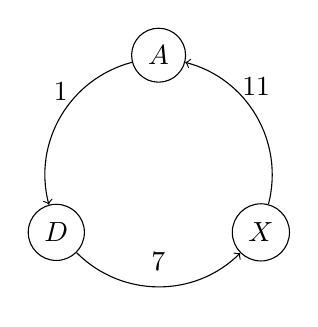
\begin{tikzpicture}[node distance=1cm, every node/.style={draw, circle, minimum height=0.1cm, minimum width=0.1cm}]
        \node (A) at (90:1.5) {$A$};
        \node (D) at (210:1.5) {$D$};
        \node (X) at (330:1.5) {$X$};
      
        \draw[->, bend right=45] (A) to node[midway, draw=none, above] {1} (D);
        \draw[->, bend right=45] (D) to node[midway, draw=none, above] {7} (X);
        \draw[->, bend right=45] (X) to node[midway, draw=none, above] {11} (A);
      \end{tikzpicture}
\end{center}

Recall
\begin{align*}
    E_1 &= P^{-1}\theta_1R_1^{-1}\theta_1^{-1}R_2^{-1}R_3^{-1}MR_3R_2\theta_1^{-1}R_1\theta_1P
    \\E_7 &= P^{-1}\theta_7R_1^{-1}\theta_7^{-1}R_2^{-1}R_3^{-1}MR_3R_2\theta_7^{-1}R_1\theta_7P
    \\E_{11} &= P^{-1}\theta_{11}R_1^{-1}\theta_{11}^{-1}R_2^{-1}R_3^{-1}MR_3R_2\theta_{11}^{-1}R_1\theta_{11}P
\end{align*}
Then it follows that our loop can be represented by 
\begin{align*}
    \sigma &= E_{11}\circ E_7 \circ E_{1}
\end{align*}
and we see that all the intermediate plugboard settings cancel out. Lets isolate the plugboard settings by letting 
$\overline{\sigma}$ represent $\sigma$ without the use of the plugboard for input and output, then 
\[
    \sigma = P^{-1}\overline{\sigma}P
\]
We have that
\begin{align*}
    \sigma(A) &= A
    \\\iff (P^{-1}\overline{\sigma}P)(A) &= A
    \\\iff \overline{\sigma}(P(A)) &= P(A)
\end{align*}

Suppose that our initial rotor position was correct, then certainly our $\overline{\sigma}$ is correct. We can make a hypothesis 
that $A$ is steckered to $K$ in the plugboard. Suppose we find that $\overline{\sigma}(K) \ne K$, then $\sigma(A)\ne A$ and our loop is broken, breaking our assumptions, thus $A$ must not be steckered to $K$.
But this will actually elimiate more hypotheses than just $A$ being steckered to $K$. We know that $\overline{\sigma}(K)$ is some letter which is not $K$. So we continue with a new hypothesis that $A$ is steckered to 
$\overline{\sigma}(K)$ and if we find $\overline{\sigma}(\overline{\sigma}(K)) \ne \overline{\sigma}(K)$, then we have further eliminated this possibility. 
Each new hypothesis suggests that $A$ is steckered to $\overline{\sigma}^{i}(K)$ which will be shown to be false if $\overline{\sigma}^{i+1}(K) \ne \overline{\sigma}^{i}(K)$. What if we find that 
$\overline{\sigma}^{i+1}(K) = \overline{\sigma}^i(K)$ at some point? This cannot happen since 
\begin{center}
        \begin{align*}
            &\overline{\sigma}^{i+1}(K) = \overline{\sigma}^i(K)
            \\\Rightarrow \text{ }&\overline{\sigma}^{-i}\circ\overline{\sigma}^{i+1}(K) = \overline\sigma^{-i}\circ\overline{\sigma}^i(K)
            \\\Rightarrow \text{ }&\overline{\sigma}(K) = K
        \end{align*}
\end{center}
which by supposition is false. Then we can continue in our hypotheses until we eventually reach a cycle where $\overline\sigma^i(K) = K$.
Then we gather a set of impossible steckerings, that is
\begin{align*}
    P(A) \notin \{\text{ }\overline{\sigma}^i(K)\text{ }\vert\text{ }i\in\mathbb{N}\}
\end{align*}
\\\\The notation we are using can be simplified significantly. The set $\{\text{ }\overline{\sigma}^i(K)\text{ }\vert\text{ }i\in\mathbb{N}\}$ is equivalent to the orbit of $K$ via the group action of the 
cyclic subgroup $\langle\overline{\sigma}\rangle$ which can be denoted $\langle\overline{\sigma}\rangle\cdot K$. 
\\\\We then have several cases 
\begin{enumerate}
    \item If $|\langle\overline{\sigma}\rangle\cdot K| = 26$, then $A$ cannot be steckered to anything which is clearly
    impossible, thus our rotor position must be incorrect. 
    \item If $|\langle\overline{\sigma}\rangle\cdot K| = 25$, then $A$ can only be steckered to the remaining letter \\$\{A,\dots,Z\} -
    \langle \overline{\sigma} \rangle\cdot K$
    \item If $|\langle\overline{\sigma}\rangle\cdot K| = 1$, in this case we must have intially had $\overline{\sigma}(K) = K$ so we have not
    eliminated any possibilities. 
\end{enumerate}